\documentclass[]{article}
\usepackage{graphicx}

\begin{document}

\title{Analyzing the Number of Updates Sent}
\maketitle
\newpage
The topology used is shown below. \\
\linebreak

\begin{center}
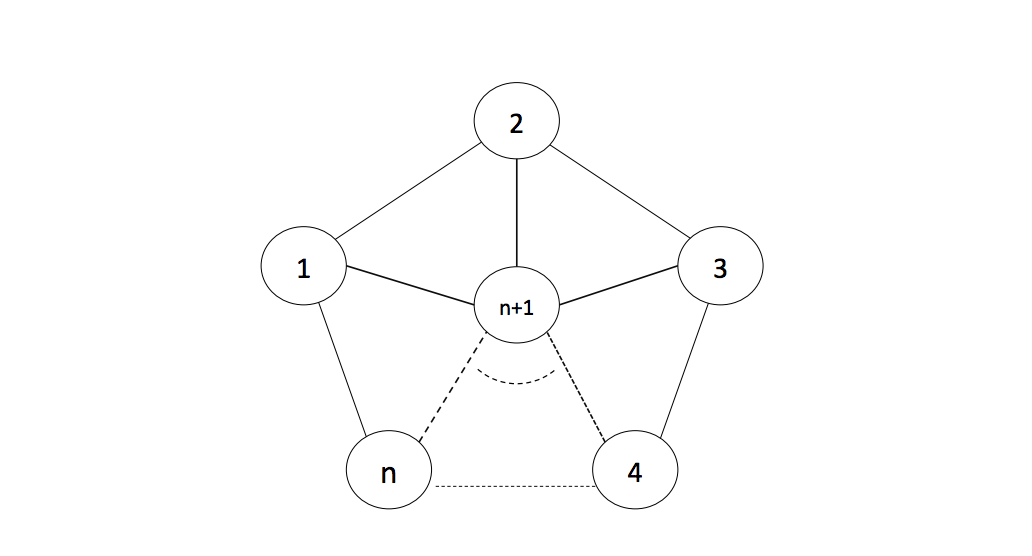
\includegraphics[width=10cm]{topo.png}
\linebreak
The total number of updates sent as a function of the number of routers in the topology is contained in the array: 

[12
16
21
26
32
36
42
48
51
56
64
65
69
75
80
86
90
92
97
105
108
113
116
123
131
132
139
141
146
150
161
162
163
175
177
176
186
186
189
204
205
220
217
213
216
220
229
229]
\linebreak

The plot of this data is shown below.
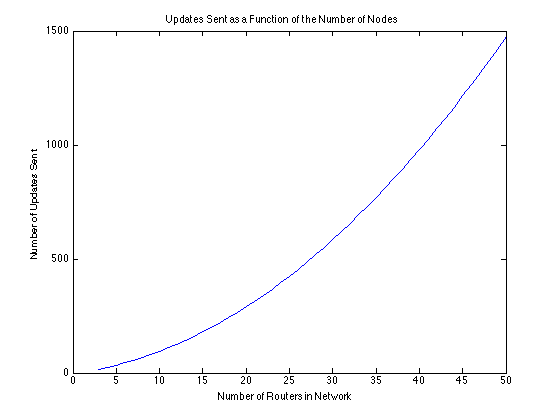
\includegraphics[width=13cm]{plot.png}
\linebreak
As we can see, with my RIPRouter implementation, the number of updates sent is relatively few and grows linearly as the number of routers in the network grows. This is fantastic, as we have a convergence time that scales proportionally with the number of routers in the network.
\end{center}
\end{document}